\section{Proposed Approach}\label{sec:approach}
A high-level description of a skip list has already been introduced in the previous section. The implemented skip list is similar to the ones proposed by \cite{Herlihy:2008:AMP:1734069, Sundell:2005:FLC:1073765.1073770}. While \cite{Herlihy:2008:AMP:1734069} uses Java and its \textit{AtomicMarkableReference}, we used C++11 and its atomic operations. Since C++11 does not provide an atomic markable reference object, we implemented our own, such that we can check a change of the reference or the mark in a single Compare-and-Swap (CAS) operation. For obtaining such a reference, multiple implementation alternatives are possible: using a bit of the pointer as a mark, double CAS, double-width CAS, and Transactional-Memory.

For our concurrent priority queue, we implemented an \textit{AtomicMarkableReference} object, by using the least significant bit as a mark. Thereby we are able to use the C++11 {\em compare\_and\_exchange} operation and are not relying on double CAS or Transactional-Memory which are less common hardware features.
In general, using the least significant bit as a mark does not lead to any issues since most 64\,bit processors only allow read or write operations from addresses which are a multiple of 8\,bytes.
As consequence the less significant bit is zero and unused.

In addition to the common skip list methods (e.g. empty, size, find, remove, and insert), we added a \textit{pop} method, which is required for a priority queue~\cite{Herlihy:2008:AMP:1734069}, and also batch processing methods for pushing or popping \textit{k} elements.

The implementation for \textit{pop} is straightforward in our concurrent priority queue, since the element with the highest priority is always located in the beginning of the skip list.
Therefore a batch \textit{pop} operation has a complexity of $\Theta(k)$. This means no significant performance improvement can be achieved over the regular \textit{pop} operation. On the other hand a batch push operation can be implemented which has some benefits over the single element operation. Since the batch push operation assumes that the input is already sorted, it is able to insert ranges of the input array instead of single elements. Thereby the number of atomic operations is reduced. In the worst case, when each range holds only one element, the batching operation behaves similar to the regular push operation.

%The interface of our implementation is shown in Listing \ref{lst:ppq-interface}.

%\begin{lstlisting}[language=C++,basicstyle=\tt\footnotesize,captionpos=b,caption=PPQ interface,morekeywords={*, size_t},label=lst:ppq-interface]
%template <class T, class Comp> class PPQ
%{
%	bool empty() const;
%	size_t size() const;
%	bool push(const T& data);
%	size_t push(T data[], int k);
%	bool remove(const T& data);
%	bool pop_front(T& data);
%	size_t pop_front(T data[], int k);
%	bool contains(T data);
%	void print();
%};
%\end{lstlisting}
\subsection{Correctness verification}
\label{subsec:corr_ver}
Two different applications were used for verifying the correctness of our concurrent priority queue.
A lossless data compression algorithm and a shortest path algorithm. 
%\mypar{Huffman coding algorithm}
First, the Huffman encoding algorithm was used to test the correctness for a single-threaded execution. The algorithm was implemented in a way that can use either an existing min-heap implementation or our own priority queue implementation.
To verify correctness, the outputs of the two variations were compared for a variety of inputs.\\
A second correctness test was based on a concurrent shortest path algorithm which is provided as an example with the Intel TBB source code.
It originally utilizes the TBB concurrent priority queue, but we adapted the algorithm to also use our own lock-free implementation.
In comparison to the previous test, this application accesses the priority queue concurrently.
Again the outputs for different input graphs of the two versions were compared to verify correctness.

Performance benchmarks for these algorithms were not conducted, since it might have implied tuning the algorithms themselves.
Such optimizations are out of the scope of this project.
In section~\ref{sec:exp}, performance evaluation against TBB concurrent priority queue, is presented for specific workloads.

\subsection{Memory allocation micro-benchmark}
\begin{figure}[t]
	\centering
	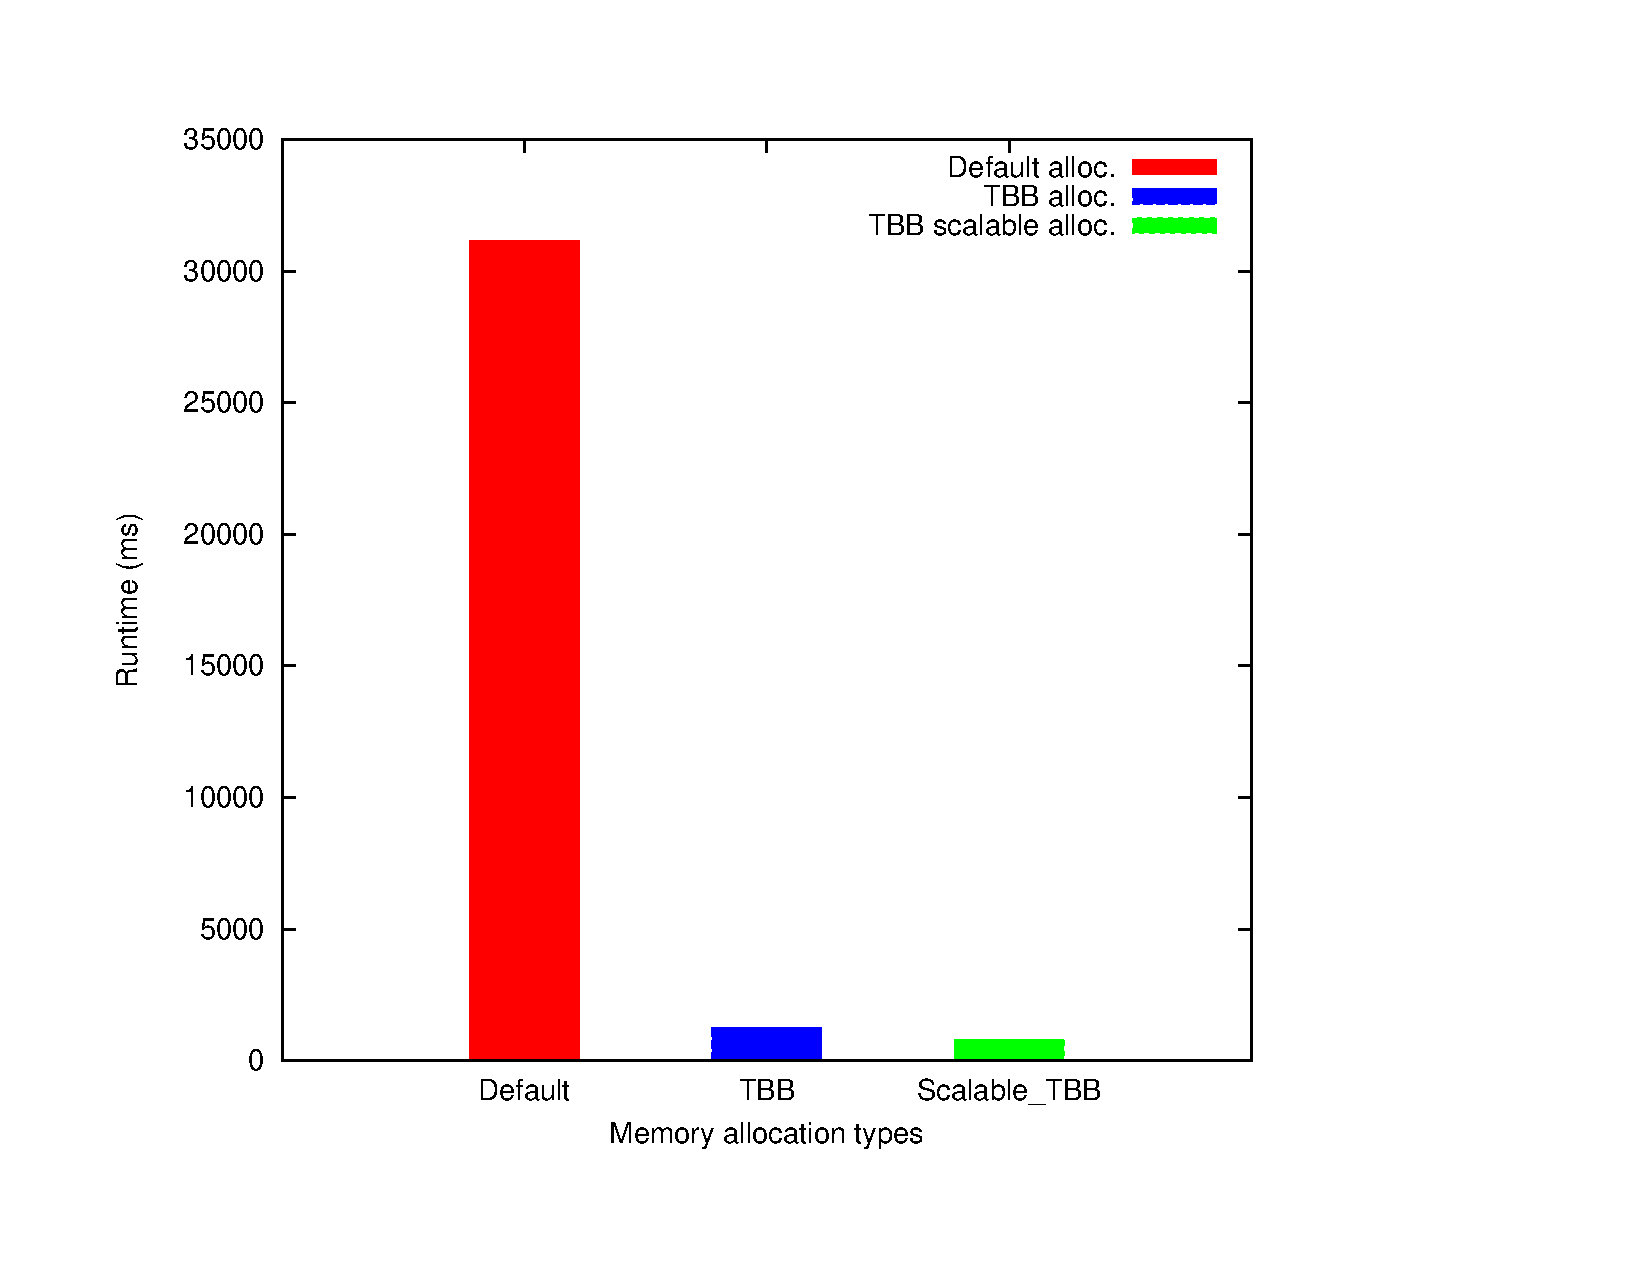
\includegraphics[scale=0.3]{../plots/mem_alloc/mem_alloc.pdf}
	\caption{Runtime allocating 10\,Mio elements using C++ default, TBB default and TBB scalable allocator.}
	\label{fig:mem_alloc}
\end{figure}

Early overall measurements indicated that memory allocation on a Xeon Phi might represent a significant part of the runtime.
Therefore, we performed a memory allocation benchmark on the Xeon Phi.
Three different allocators were considered: the default C++ allocator, the default TBB allocator and the TBB scalable allocator. 

TBB's scalable allocator is worth describing as many external applications can benefit from it.
This allocator uses a global memory heap, and provides each thread its own memory heap in order to reduce the amount of code for synchronization, and for avoiding false sharing. Then each thread accesses its own memory heap through thread-specific data, using system APIs. The allocator gets 1\,MB chunks from the operating system and divides them into 16\,KB aligned blocks. Then, it initially places these blocks in a global heap of free blocks. Memory request from the application get served from this heap, if the thread private heap does not hold any more free blocks.
In addition to that, the global heap re-uses memory blocks, by keeping freed ones from the application instead of returning them directly to the operating system.
In case a thread does not find free objects within its own heap and there are no available blocks in the global heap, additional blocks are requested to the operating system~\cite{_thefoundations,Hudson:2006:MST:1133956.1133967}. 

Our micro-benchmark consists of allocating ten million skip list nodes with 240 threads and measuring the time it takes to accomplish this task on the Xeon Phi.
As expected, the C++ default allocator has a much higher runtime than the two TBB allocators. These two allocators obtained a 24x and 38x improvement, respectively, over the C++ default allocator. The results are displayed in Fig.~\ref{fig:mem_alloc}.

While running this micro-benchmark, we observed that the core running the operating system shows a very high utilization which means that if many cores want to allocate memory they are also bound by the single core hosting the operating system.
